\header{
    \headtitle{Mon ancêtre Gurdil} \label{mon-ancetre-gurdil}
    %
    \insertComment{Chanson de Pen of Chaos (2003) tirée de l'univers de Naheulbeuk, interbrétée par le Naheulband.}{}
}

\enluminure{2}{\href{https://www.youtube.com/watch?v=UWPdBI9FlTg}{V}}{oici} l'histoire d'un nain capable
\\De courir vite, et de voyager loin
\\Dans son épopée formidable,
\\Nous le suivrons, une bière à la main !
\\\\\textbf{Refrain :}
\\Nous sommes les nains sous la montagne,
\\On creuse le jour, on boit la nuit,
\\Et on n'aime pas ceux d'la surface
\\\\Un jour, mon ancêtre Gurdil 
\\Fut envoyé creuser dans la forêt,
\\Y'avait soi disant du mithril,
\\Si y'en avait on sait pas où il s'trouvait
\\Il fit sa cabane en bordure,
\\D'un bois touffu, peuplé d'elfes sylvains,
\\Des gens qui bouffent de la verdure,
\\Évidemment ça n'fait pas de bons voisins.
\\\\Arrière tu n'es pas bienvenu
\\Lui dirent les elfes, en lui jetant des pierres,
\\Voyant que tout était foutu,
\\Il prit la fuite, en suivant la rivière,
\\Il fut recueilli par les fées,
\\Ondines bleues, bullant sur le rivage,
\\De l'eau de pluie lui fut donnée,
\\Il recracha (pfoua !) tout dans leurs visages
\breakpage
Courant à travers les fougères,
\\Il arriva, près d'un village humain,
\\Bien sûr qu'on y vendait d'la bière,
\\Mais aucun homme ne voulait servir un nain!
\\Gurdil, massacra le patron
\\D'une taverne, à coups de tabouret
\\Puis il rentra a la maison,
\\Et de la mine il ne repartit jamais!
\\\\Amis restons bien a l'abri,
\\Mangeons buvons, dans nos maisons de pierres
\\Là-haut, c'est peuplé d'abrutis
\\Allez patron, ressers donc une bière
\\\\\textbf{Refrain x2}
\bigskip
\bigskip
\begin{center}
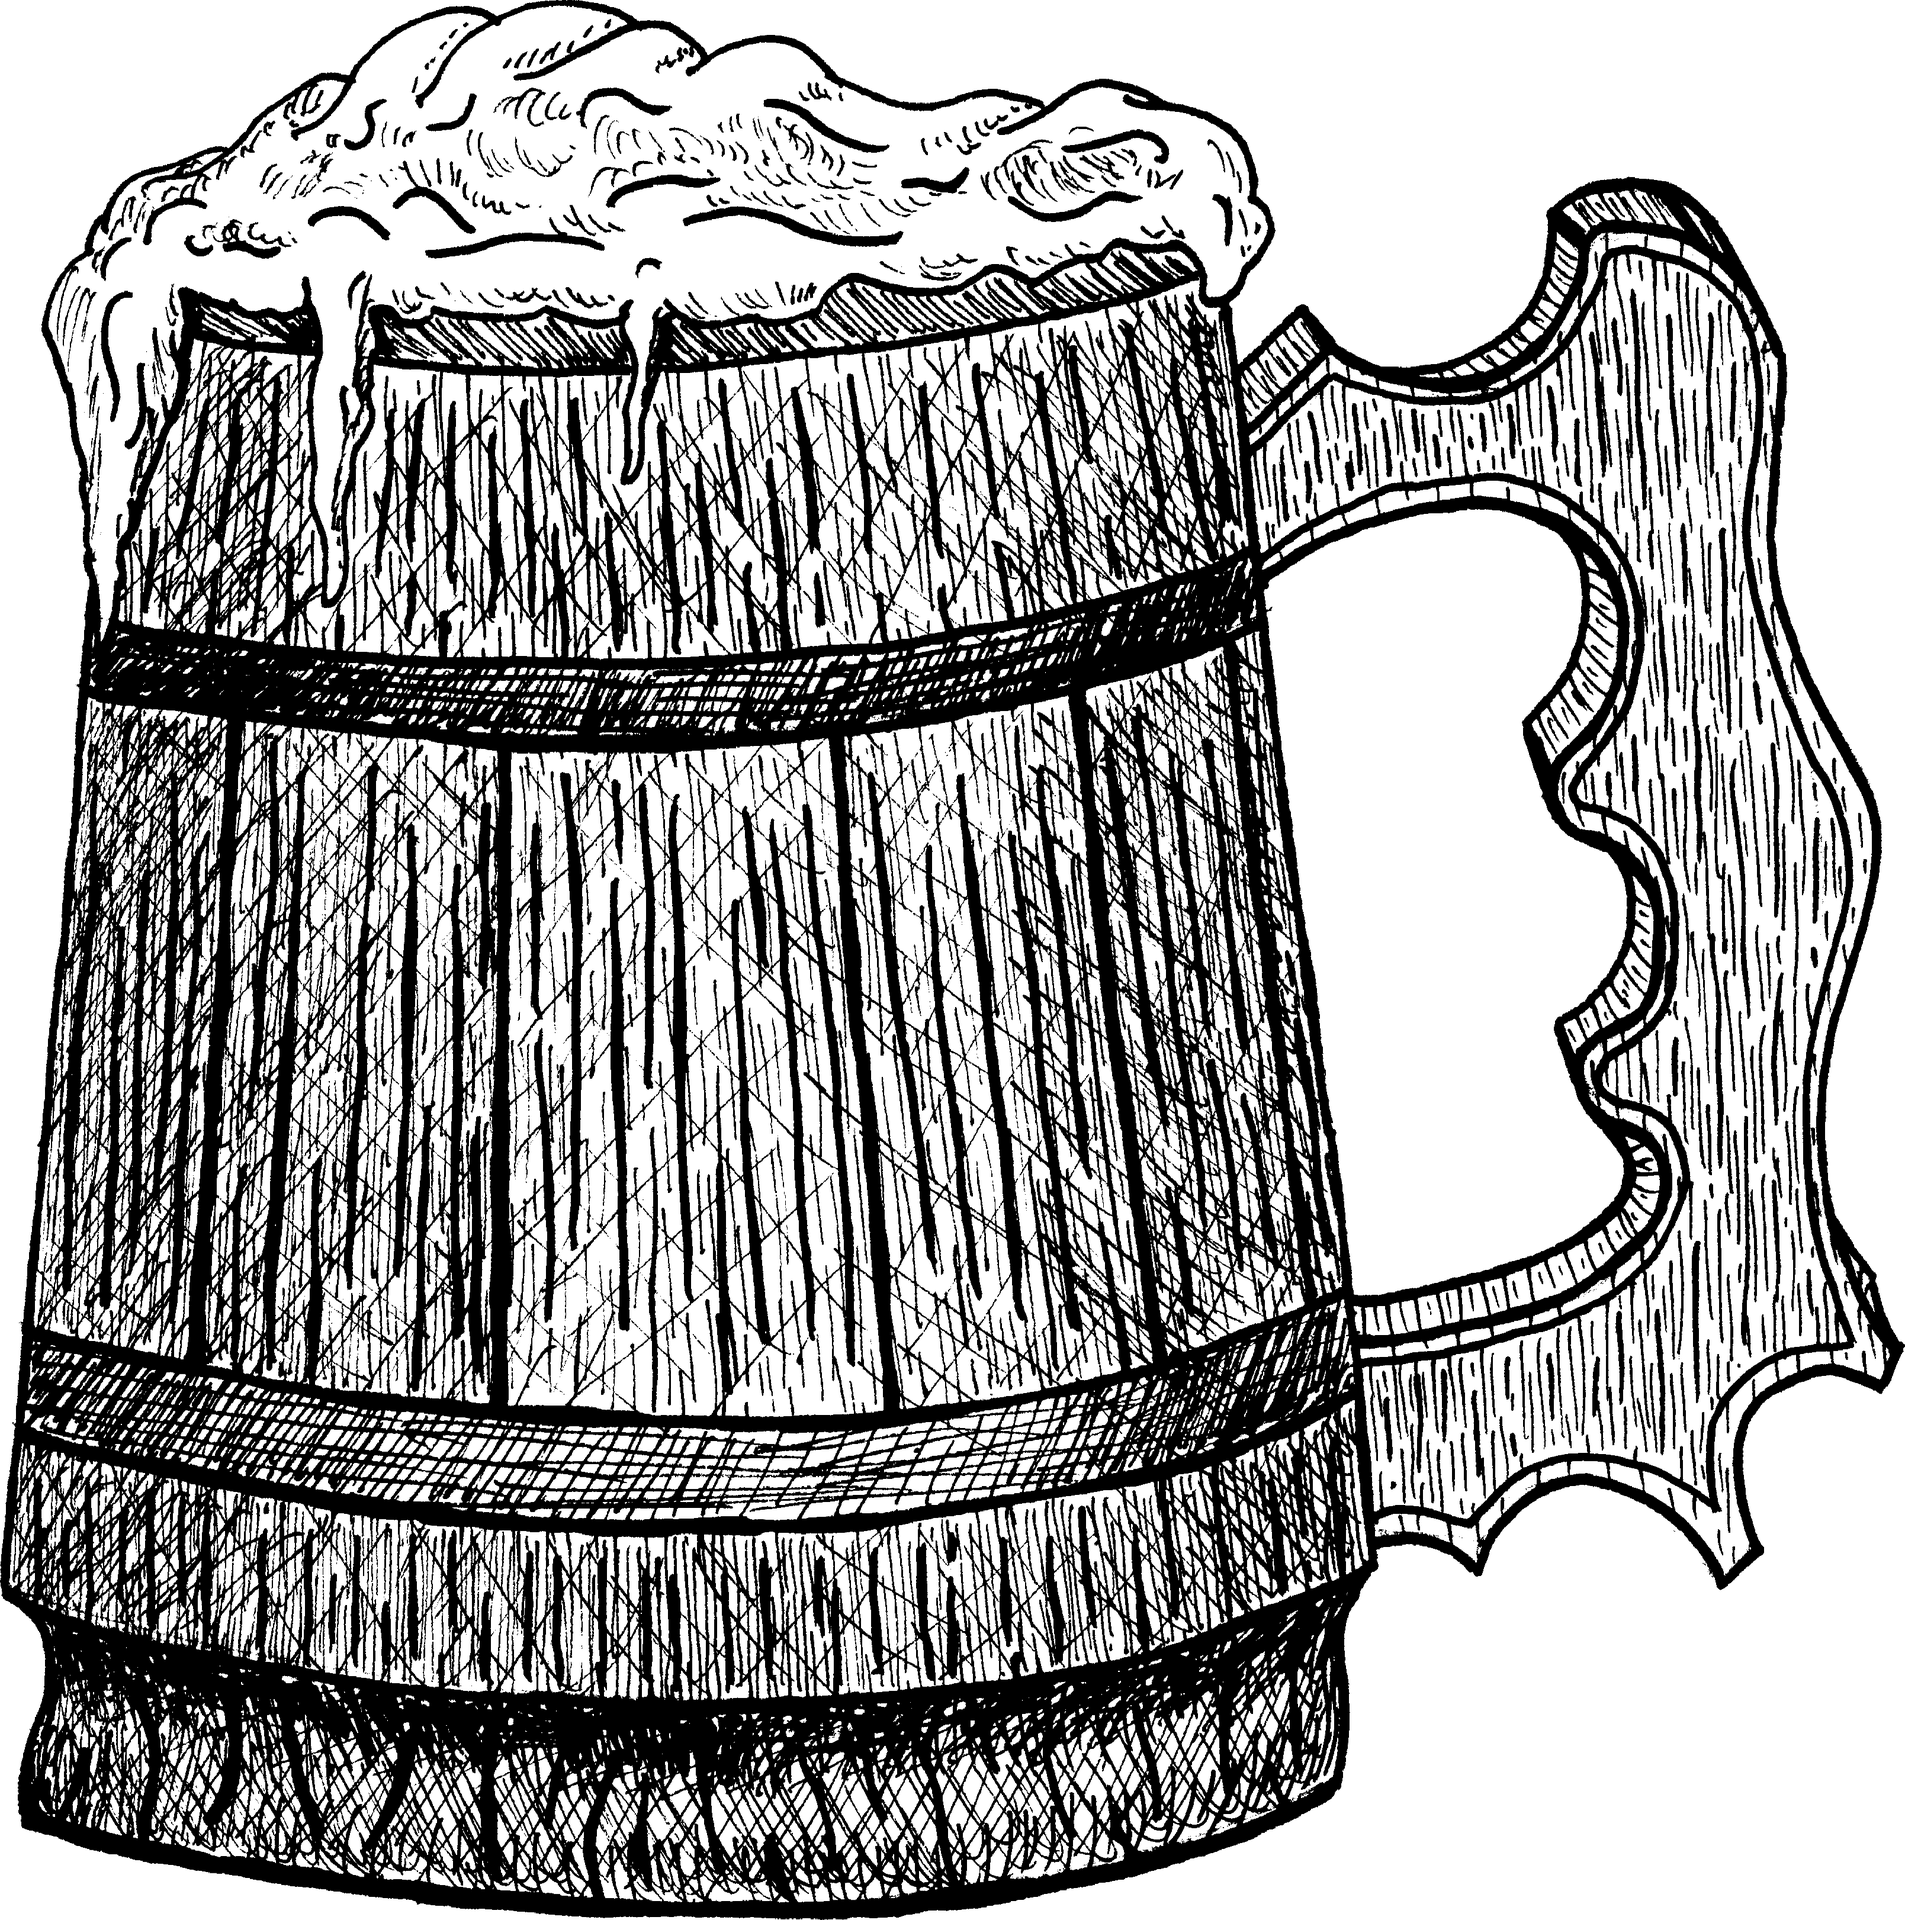
\includegraphics[width=0.8\textwidth]{images/brev65.png}
\end{center}
\breakpage